\documentclass{article}
\usepackage[utf8]{inputenc}
\usepackage{graphicx}
\usepackage[figurename=Figure]{caption}
\usepackage{float} 
\usepackage{verbatim}
\usepackage{verbatim}
\usepackage{amssymb}
\usepackage{fullpage} 
\usepackage{paralist}
\usepackage{listings}
\usepackage{subfig}
\usepackage{enumitem}
\usepackage{bm}
\usepackage{booktabs} %professional-quality tables
\usepackage{hyperref}
\hypersetup{
    colorlinks=true,
    linkcolor=blue,
    urlcolor=magenta,
}
\renewcommand{\baselinestretch}{1.15}
\setlength{\parindent}{1em}
\setlength{\parskip}{0.1mm}

\begin{document}
\title{\textbf{Sampling Term Project}}\\
\date{November.13, 2020} 



\maketitle
\newpage
\section{Introduction}
\textbf{Objective:} \\

In this project, we aim to explore the average number of full-time equivalency(FTE) students as well as the proportion of percentage of International students in all universities around the world. \\

\noindent\textbf{Background:} \\

Various studies have suggested continuing growth in the global demand for higher education; at the same time the number of university enrollments has been rapidly increased in recent years. Also, the rates of international students among universities have been increased along with the development of the country. 

Exploring the average number of full-time equivalency enrollments of all universities and the percentage of international students can help us investigate the education level of the whole world or of different continents specifically. In addition, international students represents a country’s soft power and economic level to certain extent. 

Furthermore, we also interested in the preferences of international students in terms of choosing their academic institutions for studying aboard. \\

\noindent\textbf {Data Obtaining:} 
\href{https://www.timeshighereducation.com/world-university-rankings/2020/world-ranking#!/page/0/length/25/sort_by/rank/sort_order/asc/cols/stats}{Reference: Times Higher Education World University Rankings 2020} \\

\noindent\textbf {Targeted population:} \\

All universities listed on the Times Higher Education World University Rankings 2020. This detailed ranking list includes almost 1400 universities across 92 countries.  \\

\noindent\textbf {Parameter of interest:} \\

\noindent continuous variable: the full-time equivalency(FTE) enrollment number of a university \\
binary variable: whether the percentage of international students is over 15\% in a university \\

\noindent\textbf{Sampling methods:} Simple Random Sampling (SRS) and Stratified Sampling. \\

\noindent\textbf{SRS:} We randomly obtain a sample of size 100 universities \\
\noindent\textbf{Stratified Sampling:} We would choose strata according to continents, thus having six strata in total:  Africa, Asia, Oceania, Europe, North America, and South America. In order to obtain the sample sizes of each strata, we calculate according to the sample allocation theorem:
$ \frac{n_h}{n}\ = \frac{N_h}{n}\ $ \\
\newpage
\section{Data collection and data summaries}
\subsection{{\textbf{\textit{Overview:}}}}\\
The source of our data is the world university ranking 2020 from Times Higher Education. We extracted the name of the university, the number of full-time efficiency students and the percentage of international students and added the country and continent of each university accordingly. 

\noindent  The data has 1397 rows, indicating 1397 universities around the world, and 5 columns, indicating information of:\\
    1. the university name (character)\\
    2. the number of full-time equivalency students in year 2020 (number)\\
    3. the percentage of international students in the university in year 2020 (number)\\
    4. the country (character) the university is located in\\
    5. the continent (character) the university is located in\\
    
\subsection{{\textbf{\textit{Data Summaries}}}}\\

\textbf{Continuous:}\\

 \begin{table}[h]
    \begin{center}
    \caption{parameter of interest: No. of FTE Students}
    \begin{tabular}{ | c| c | c | c |}
    \hline
    \multicolumn{4}{|c|}{Simple Random Sampling} \\
    \hline
    mean & se & \multicolumn{2}{|c|}{Confidence Interval} \\ 
    \hline
    21514.550 & 1479.264 & 18615.192 & 24413.908\\ 
    \hline
    \multicolumn{4}{|c|}{Stratified Sampling} \\
    \hline
    mean & se & \multicolumn{2}{|c|}{Confidence Interval} \\ 
    \hline
    20605.493 & 1313.717 & 18030.607 & 23180.379\\ 
    \hline
    \end{tabular}
    \label{tab:(a)}
    \end{center}
    \end{table}

\textbf{Binary:}

\begin{table}[h]
    \begin{center}
    \caption{parameter of interest: Proportion of International students(\%)}
    \begin{tabular}{ | c| c | c | c |}
    \hline
    \multicolumn{4}{|c|}{Simple Random Sampling} \\
    \hline
    mean & se & \multicolumn{2}{|c|}{Confidence Interval} \\ 
    \hline
    0.28000000 & 0.04326304 & 0.19520444 & 0.36479556\\ 
    \hline
    \multicolumn{4}{|c|}{Stratified Sampling} \\
    \hline
    mean & se & \multicolumn{2}{|c|}{Confidence Interval} \\ 
    \hline
    0.32027644 & 0.03912274 & 0.24359588 & 0.39695700\\ 
    \hline
    \end{tabular}
    \label{tab:(b)}
    \end{center}
    \end{table}



\newpage
\section{Data analysis}
\textbf{Continuous:}

For the number of fulltime-efficiency students in a university, the minimum number is 558 students and the maximum number is 830104 students. According to histogram in {\hyperref[fig:test4]{Figure 4}}, it could be seen that the histogram is uni-modal, and there is a peak on the left of the center, indicating a right-skewed histogram.

It is calculated that the population mean for the number of fulltime-efficiency students is 23741 with a population standard deviation of 32821, and the population median is 17848.Therefore, we would know that the mean is greater than the median.\\

\noindent{\textit{Simple Random Sampling (SRS)}:}

We treat the data as the population and first perform a Simple Random Sample. A random sample of size 100 is drawn without replacement.
The sample mean is found to be 21514.55, with a sample standard error of 1479.264, calculated from the sample variance using the formula:
$$se_{sample} = \sqrt{((1 - \frac{n}{N}) * (\frac{Var_{sample}}{n})} (with CLT)$$\\
Therefore, we calculate the confidence interval using the formula:\\
$(mean_{sample} – 1.96*se_{sample}, mean_{sample} + 1.96*se_{sample})$, and get the confidence interval of (18615.192, 24413.908) which includes the true population mean.

\noindent{\textit{Stratified Sampling}:}

We treat the data as the population, and we stratify the samples based on continents where universities are located, thus having 6 strata in total: Europe, Asia, Africa, South America, Oceania and North America, since Antarctica has no universities.
  
  The pie-chart in {\hyperref[fig:test1]{Figure 1}}
   shows the proportions of the universities in each continent in the data, and the bar-chart in {\hyperref[fig:test3]{Figure 3}} shows the total number of universities in each continent. We see that some continents have bigger proportions comparing to the others. Therefore, when choosing the sampling size within each strata, we use the sample allocation theorem of $ \frac{n_h}{n}\ = \frac{N_h}{n}\ $

According to calculation, the sample sizes of each stratum are found out as the following:

\begin{table}[h]
    \begin{center}
    \caption{Strata Data}
    \begin{tabular}{c c c c c }
Strata Name & N_h & N_h/N (N = 1397) & n & n_h \\
Asia & 493 & 0.3528 & 100 & 35 \\
Africa & 57 & 0.0408 & 100 & 4 \\
Europe & 501 & 0.3586 & 100 & 36 \\
North America & 223 & 0.1596 & 100 & 16 \\
South America & 80 & 0.0573 & 100 & 6 \\
Oceania & 43 & 0.0308 & 100 & 3
    \end{tabular}
    \label{tab:(c)}
    \end{center}
    \end{table}

After obtaining the sample sizes, we loop over the continents. First, we get the row indices corresponding to a specific continent and save the results to the said indices. Then We sample the indices to get the corresponding rows from the population data. Finally we add the sample for this stratum to those from the previous strata.

The sample mean $mean_{str}$ is found to be 20605.493, the sample standard error $se_{str}$ is found to be 1313.717. 

The standard error within each stratum is: \\
$$se.prop_{str} = \sqrt{(1-\frac{n_h}{N_h}) * (\frac{var,prop_{str}}{n_h})}$$, and the sample standard error is calculated using the formula:\\
$$se_{str} = \sqrt{(\sum_{h=1}^{H = 6}(\frac{N_h}{N})^2*str_{se}^2))}$$ 

According to the formula $(mean_{str} – 1.96*se_{str}, mean_{str} + 1.96*se_{str})$, the confidence interval is calculated to be (18030.607, 23180.379), which does not contain the true population mean. \\

\noindent{\textit{Results Interpretation:}}

According to the estimates in {\hyperref[tab:(a)]{Table 1}}, stratified sampling provides a smaller standard error compared to simple random sampling , resulting in a narrower confidence interval. While in the simple random sample, the confidence interval managed to include the true population mean while the stratified sampling has not.\\

\noindent{\textbf{Binary}:}\\

 For the percentage of international students in universities, the minimum is 0\% and the maximum is 83\%. It is calculated that the population mean for the international students rates is 0.2749 with a population standard deviation of 0.4466.\\

 A new binary variable called "Binary" is created, indicating whether the proportion of international student(\%) in a university is greater than 0.15 or not. If the rate is larger than 0.15, we set the Binary to 1; otherwise, we set the Binary to 0. We found that among 1397 universities, there are 384 of them have more than 15 percent of international students, and 1013 of them do not, which can be seen in {\hyperref[fig:test2]{Figure 2}}, the proportion of universities with more than 15\% international students is smaller than the proportion of universities with less than or equal to 15\% international students.\\

\noindent{\textit{Simple Random Sampling (SRS)}:}

We treat the data as the population and first perform a Simple Random Sample. A random sample of size 100 is drawn without replacement.

The sample mean $\hat{p}$ is found to be 0.2800, with a sample standard error $se_{sample2}$ of 0.04326, calculated with the formula:
$$se_{sample2} = \sqrt{(1-\frac{n}{N})*\frac{\hat{p}*(1-\hat{p})}{n}}$$
Therefore, we use the formula: $(\hat{p}_{sample2} – 1.96 * se_{sample2}, \hat{p}_{sample2} + 1.96 * se_{sample2})$, to calculate the confidence interval of (0.1952, 0.3648), which covers the true population mean.\\

\noindent{\textit{Stratified Sampling}:}

We treat the data as population, and we stratified the sample by continents as well. 

The sample sizes of each stratum are obtained the same way as the stratified sample above, as {\hyperref[tab:(c)]{Table 3}} shown.

The sample mean $\hat{p}_{str2}$ is found to be 0.3203. The standard error within each stratum is 
$$se.prop_{str2} = \sqrt{(1-\frac{n_{h2}}{N_{h2}})* \frac{\hat{p}.prop_{str2}*(1-\hat{p}.prop_{str2})}{n_{h2}}}$$.  Then we calculate the sample standard error by using the formula:
$$se_{str2} = \sqrt{\sum_{h=1}^{H=6}(\frac{N_{h2}}{N})^2 * se.prop_{str2}^2)}$$ and the value of the standard error STR.se2 is 0.03912. 

According to the formula $($\hat{p}_{str2}$ – 1.96*se_{str2},  $\hat{p}_{str2}$ + 1.96*se_{str2})$, we found that the confidence interval is (0.2436, 0.3970), which covers the population mean. \\

\noindent\textit{Results Interpretation:}

According to the estimates in {\hyperref[tab:(b)]{Table 2}}, for the stratified sampling we use, the standard error is still smaller then the standard error of simple random sampling's. We can see that both the SRS estimate and the STR estimate covers the true population mean; However, it takes more work to pull a stratified sample than a random sample. \\

\noindent{\textbf{Advantage and Disadvantage of the Sampling methods:}}

The advantage of using simple random sampling is that the sample is easy to obtain, with only one simple step. As well, each individual in the population has an equal chance to be selected, thus there is more fairness involved. 

However, there is a risk of over representation or under representation of particular patterns or variations resulting in a greater risk of data manipulation. Moreover, both standard errors in the two SRS simulations appears to be quite large. Thus, the SRS estimates can be inaccurate when predicting population. 

In stratified sampling, since we divided the population into 6 different strata and used proportional allocation to assign strata sample sizes, the standard error in stratified sampling is smaller than that in SRS, indicating a greater precision and a more representative sample. Furthermore, it could be ensured that sufficient samples are obtained to support analysis of any subgroup (stratum).

However, looking at the computation, the calculation of stratified sampling appears to be more complex than simple random sampling. Also, for each strata-since we are using SRS to select sample units in each strata-the same problem occurs: although each university in one continent has an equal chance to be selected, but the sample data can still be biased and result in an inaccurate approximation of the population.



\section{Conclusions and discussion}

According to the results from {\hyperref[tab:(a)]{Table 1}} and {\hyperref[tab:(b)]{Table 2}}, we could generalize that stratified sampling results in smaller standard error and narrower 95\% confidence interval than simple random sample. The reason, in short, is stratified sampling ensures each domain within the population has proper representation in the sample compared to pure simple random sampling, and thus provides better coverage of the population . In, this study, stratified sampling, instead of doing pure simple random sampling, we consider one more variable(continents) and acquire samples which are more representative than simple random samples. Therefore, stratify sampling offers greater preciseness of estimation in both continuous and binary variables.

Limitation of our study is sample data bias. Although we testified stratified sampling is more accurate than simple random sampling, it is because for stratified sampling, instead of doing pure simple random sampling, we consider one more variable(continents) and acquire samples which are more representative than simple random samples. However, after we divided the strata and determined the sample sizes for each strata, we still used SRS to acquire each strata sample. Thus, the limitation with both SRS and STR sampling is we are not able to avoid sample data bias completely.

Other limitations should also be noted. First, The data we obtained was universities specifically listed in Times World University Rankings. Since we are interested in all universities around the world, we noticed that not every university in the world is included in this ranking, which could induce that this study may not be applicable to universities outside of this designation. Second, as discussed above, data bias is existing. Specifically, after we divided the strata and determined the sample sizes for each strata, we still used SRS to acquire each strata sample. Thus, the limitation with both SRS and STR sampling is we are not able to avoid sample data completely.


\section{Appendix}
\subsection{\textbf{\textit{Data Source:}}}
\textit{The Times Higher Education} World University Rankings 2020\\
\url{https://www.timeshighereducation.com/world-university-rankings/2020/world-ranking#!/page/0/length/25/sort_by/rank/sort_order/asc/cols/stats}

\subsection{\textbf{\textit{Code Written:}}}
\underline{Continuous Population:}

\noindent\textit{Simple Random Sampling:}\\
\textgreater\hspace{1mm} universitydata \textless- read \textunderscore excel("Desktop/STAT 344/project/universitydata.xlsx")    \# reading data\\
\textgreater\hspace{1mm} summary(univeristitydata)    \# summary statistics for each variable
\begin{figure}[htp]
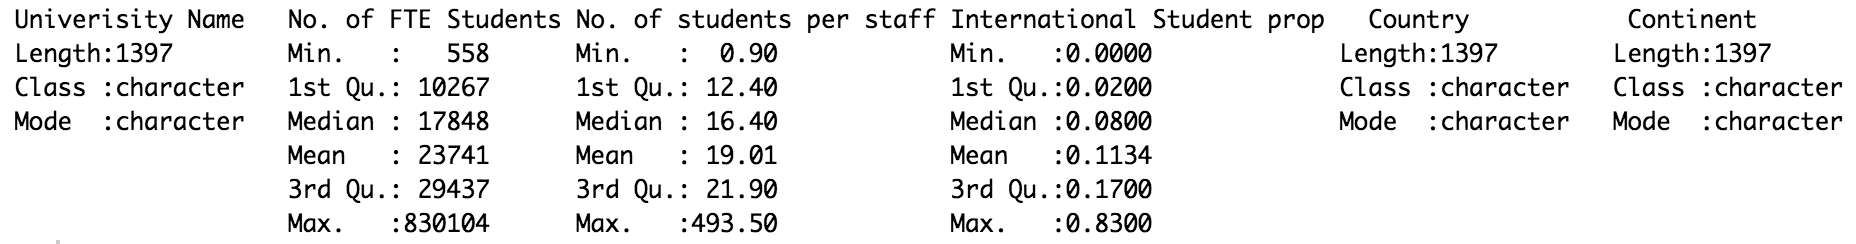
\includegraphics[width=18cm]{summarydata.png}
\label{lable:sunmary}
\end{figure} \\
\textgreater\hspace{1mm} pop.mean \textless- mean(universitydata\textdollar`No. of FTE Students`)~~ \# population mean of FTE students\\
  23741.15\\
\textgreater\hspace{1mm}pop.sd \textless- sd(universitydata\textdollar `No. of FTE Students`) \# population sd of FTE students\\
  32821.3\\
\textgreater\hspace{1mm} N \textless- nrow(universitydata)~~~~~~ \# population size N\\
\textgreater\hspace{1mm} n \textless- 100 ~~~~~~~~~~~~~~~~~~~~~~~~~~~~~~ \# sample size n (100)\\
\textgreater\hspace{1mm} SRS.indices \textless- sample.int(N, n, replace = F)\\
\textgreater\hspace{1mm} SRS.sample \textless- universitydata[SRS.indices, ] ~~~~~~~~~~~~~~~~~~~~\# sample\\
\textgreater\hspace{1mm} SRS.mean \textless- mean(SRS.sample\textdollar`No. of FTE Students`)~~~~ \# sample mean\\
\textgreater\hspace{1mm} SRS.sd \textless- sqrt(var(SRS.sample\textdollar`No. of FTE Students`)) ~~~~\# sample sd\\
\textgreater\hspace{1mm} SRS.se \textless- sqrt((1-n/N)/n)*SRS.sd ~~~~~~~~~~~~~~~~~~~~~~~~~~~~~~~~~\# sample se\\
\textgreater\hspace{1mm} SRS.CI \textless- c(SRS.mean-1.96*SRS.se, SRS.mean+1.96*SRS.se) \# calculate 95\% CI for population mean\\
\textgreater\hspace{1mm} SRS \textless- c(SRS.mean, SRS.se, SRS.CI) \# estimates\\
\hspace{1mm} 21514.550  1479.264 18615.192 24413.908\\

\noindent\textit{Stratified Sampling:}\\
\textgreater\hspace{1mm} attach(universitydata)\\
\textgreater\hspace{1mm} N.h \textless- tapply(`No. of FTE Students`, Continent, length) ~~ \# population sizes for different strata(continents) \\
\textgreater\hspace{1mm} continents \textless- names(N.h)\\
\textgreater\hspace{1mm} n.h.prop \textless- round((N.h/N)*n) ~~~~~~~~~~ \# sample sizes for each continent\\
\texttgreater\hspace{1mm} detach(universitydata)\\
\textgreater\hspace{1mm} STR.sample.prop \textless- NULL\\
\hspace{1mm} \# estimate the population mean using STR with proportional allocation\\
\textgreater\hspace{1mm} for(i in 1: length(continents)) \\
\textbraceleft\\
row.indices \textless- which(universitydata\textdollar Continent == continents[i])\\
sample.indices \textless- sample(row.indices, n.h.prop[i], replace = F)\\
STR.sample.prop \textless- rbind(STR.sample.prop, universitydata[sample.indices, ]))\\
\textbraceright\\
\hspace{1mm} \# sample mean of each stratum\\
\textgreater\hspace{1mm} STR.mean.prop \textless- tapply(STR.sample.prop\textdollar `No. of FTE Students`, STR.sample.prop\textdollar Continent, mean)\\
\hspace{1mm} \# sample variance of each stratum\\
\textgreater\hspace{1mm} STR.var.prop \textless- tapply(STR.sample.prop\textdollar `No. of FTE Students`, STR.sample.prop\textdollar Continent, var)\\
\hspace{1mm} \# sample standard error of each stratum\\
\textgreater\hspace{1mm} STR.se.prop \textless- sqrt((1-n.h.prop/N.h)*STR.var.prop/n.h.prop)\\
\hspace{1mm} \# sample 95\% CI of each stratum\\
\textgreater\hspace{1mm} STR.CI.porp \textless- c(STR.mean.prop-1.96*STR.se.prop, STR.mean.prop+1.96*STR.se.prop)\\
\textgreater\hspace{1mm} STR.mean \textless- sum(N.h / N * STR.mean.prop) ~~~~~~~~~~~~~~~~~~~~~~~\# sample mean\\
\textgreater\hspace{1mm} STR.se \textless- sqrt(sum((N.h / N)\textasciicircum 2 * STR.se.prop\textasciicircum 2)) ~~~~~~~~~~~~~~~~\# sample se\\
\textgreater\hspace{1mm} STR.CI \textless- c(STR.mean-1.96*STR.se, STR.mean+1.96*STR.se) \# calculate 95\% CI for population mean\\
\textgreater\hspace{1mm} STR.prop \textless- c(STR.mean, STR.se, STR.CI) ~~~~~~~~~~~~~~~~~~~~~~~~~\# estimates\\
\hspace{1mm} 20605.493 1313.717 18030.607 23180.379\\
\noindent\underline{Binary Population:}

\noindent\textit{Simple Random Sampling:}\\
\# create a new categorial vairable Binary that indicates whether the proportion of international students is greater than 0.15, Binary = 1 if proportion is smaller or equal to 0.15, Binary = 0.\\
\textgreater\hspace{1mm} for (i in 1: length(universitydata\textdollar`International Student(\%)`))\\
\hspace{1mm} \textbraceleft\\
\hspace{1mm} if (universitydata\textdollar`International Student(\%)`[i] \textgreater0.15) \textbraceleft\\
\hspace{1mm} universitydata\textdollar Binary[i] = 1 \textbraceright\\
\hspace{1mm} else \textbraceleft universitydata\textdollar Binary[i] = 0 \textbraceright\\
\hspace{1mm}  \textbraceright\\
\# SRS\\
\textgreater\hspace{1mm} universitydata\textdcollar Binary \textless- as.numeri(universitydata\textdollar Binary)~~~\#for calculating population mean\\
\textgreater\hspace{1mm} N \textless- nrow(universitydata) ~~~~~~~~~~~~~~~~~~~~~~~~~~~~~~~~~~~~~~~~\# population size\\
\textgreater\hspace{1mm} n \textless- 100 ~~~~~~~~~~~~~~~~~~~~~~~~~~~~~~~~~~~~~~~~~~~~~~~\#sample size\\
\textgreater\hspace{1mm} binpop.mean \textleft-universitydata\textdollar Binary) ~~~~~~~~~~~~~~~~~~~~~~~\#population mean\\
\hspace{1mm} 0.2748747\\
\textgreater\hspace{1mm} sd(universitydata\textdcollar Binary) ~~~~~~~~~~~~~~~~~~~~ \#population sd\\
\hspace{1mm} 0.446611\\
\textgreater\hspace{1mm} SRS.indices2 \textless- sample.int(N, n, replace = F)\\
\textgreater\hspace{1mm} SRS.sample2 \textless- universitydata[SRS.indices2,] ~~~~~~~~~~~~~~~~~~~~~~~\#generating sample\\
\textgreater\hspace{1mm} SRS.mean2 \textless- mean(SRS.sample2\textdollar Binary) ~~~~~~~~~~~~~~~~~~~~~~~~~~\#sample mean\\
\textgreater\hspace{1mm} SRS.se2 \textless- sqrt((1-n/N)*SRS.mean2*(1-SRS.mean2)/n) ~~~~~~~~~~~~~\#sample se\\
\textgreater\hspace{1mm} SRS.CI2 \txetless- c(SRS.mean2-1.96*SRS.se2, SRS.mean2+1.96*SRS.se2) \#calculating 95\% CI\\
\textgreater\hspace{1mm} SRS2 \textless- c(SRS.mean2, SRS.se2, SRS.CI2) ~~~~~~~~~~~~~~~~~~~~~~~~~~~~~~~\#estimates\\
\textgreater\hspace{1mm} SRS2\\
\hspace{1mm} 0.28000000 0.04326304 0.19520444 0.36479556\\
\noindent\textit{Stratified Sampling:}\\
\# STR\\
\textgreater\hspace{1mm} attach(universitydata)\\
\textgreater\hspace{1mm} N.h2 \textless- tapply(Binary, Continent, length) \# population sizes for different strata(continents)\\
\textgreater\hspace{1mm} continents2 \textless- names(N.h2)\\
\textgreater\hspace{1mm} detach(universitydata)\\
\textgreater\hspace{1mm} n.h.prop2 \textless- round((N.h2/N)*n) \# sample size for each continent\\
\textgreater\hspace{1mm} STR.sample.prop2 \textless- NULL\\
\hspace{1mm} \# estimate the population mean using STR with proportional allocation\\
\textgreater\hspace{1mm} for(i in 1: length(continents2))\\
\hspace{1mm} \textbraceleft\\
\hspace{1mm} row.indices2 \textless- which(universitydata\textdollar Continent == continents2[i])\\
\hspace{1mm} sample.indices2 \txetless- sample(row.indices2, n.h.prop2[i], replace = F)\\
\hspace{1mm} STR.sample.prop2 \textless- rbind(STR.sample.prop2, universitydata[sample.indices2, ])\\
\hspace{1mm} \textbraceright\\
\hspace{1mm} \# sample mean for each stratum\\
\textgreater\hspace{1mm} STR.mean.prop2 \textless- tapply(STR.sample.prop2\texttdollar Binary, STR.sample.prop2\textdollar Continent, mean)\\
\hspace{1mm} \# sample variance for each stratum\\
\textgreater\hspace{1mm} STR.var.prop2 \textless- tapply(STR.sample.prop2\textdollar Binary, STR.sample.prop2\textdollar Continent,var)\\
\hspace{1mm} \# sample se for each stratum\\
\textgreater\hspace{1mm} STR.se.prop2 \textless- sqrt((1-n.h.prop2/N.h2)*(STR.mean.prop2*(1-STR.mean.prop2))/n.h.prop2)\\
\hspace{1mm} \# sample CI for each stratum
\textgreater\hspace{1mm} STR.CI.porp2 \textless- c(STR.mean.prop2-1.96*STR.se.prop2, STR.mean.prop2+1.96*STR.se.prop2) \\
\textgreater\hspace{1mm} STR.mean2 \textless- sum(N.h2 / N * STR.mean.prop2) \#sample mean\\
\textgreater\hspace{1mm} STR.se2 \textless- sqrt(sum((N.h2 / N)\textasciicircum2 * STR.se.prop2\textasciicircum2)) \#sample se\\
\textgreater\hspace{1mm} STR.CI2 \textless- c(STR.mean2-1.96*STR.se2, STR.mean2+1.96*STR.se2) \#sample 95\% CI\\
\textgreater\hspace{1mm} STR.prop2 \textless- c(STR.mean2, STR.se2, STR.CI2) \#estimates\\
\textgreater\hspace{1mm} STR.prop2\\
\hspace{1mm} 0.32027644 0.03912274 0.24359588 0.39695700\\

\subsection{\textbf{\textit{Figures Used:}}}

\begin{figure}
\centering
\begin{minipage}{.5\textwidth}
  \centering
  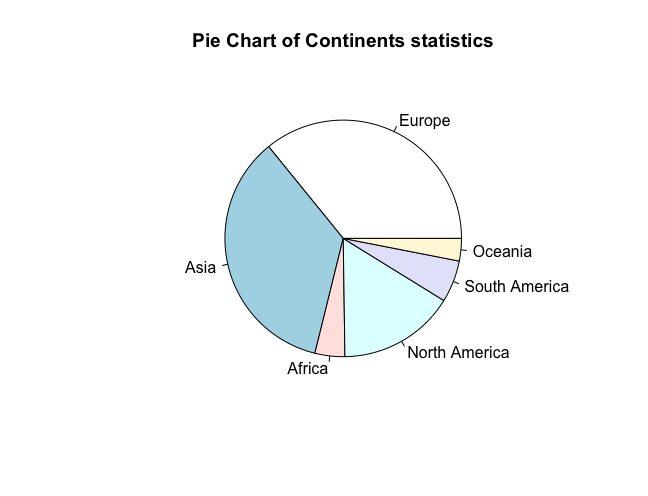
\includegraphics[width= 10cm]{Continent pie.png}
  \captionof{figure}{Pie chart of Continents statistics}
  \label{fig:test1}
\end{minipage}%
\begin{minipage}{.5\textwidth}
  \centering
  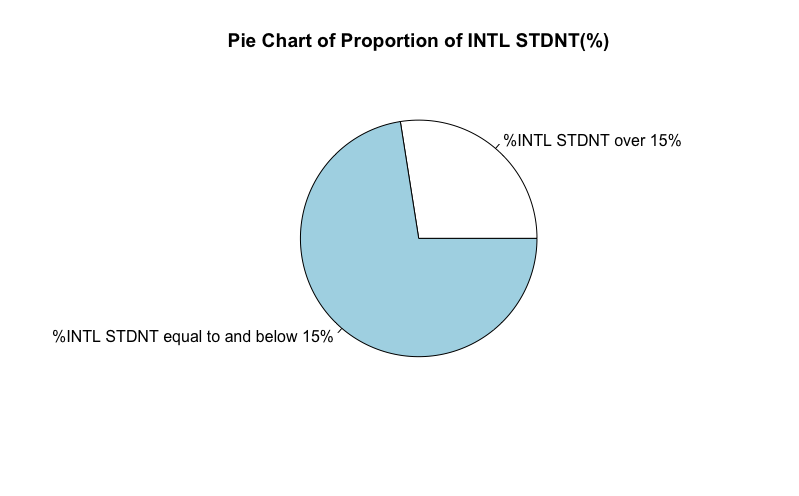
\includegraphics[width=12cm]{binary pie.png}
  \captionof{figure}{Pie chart of \%INTL STDNTS(\%)}
  \label{fig:test2}
\end{minipage}
\end{figure}

\begin{figure}
\centering
\begin{minipage}{.5\textwidth}
  \centering
  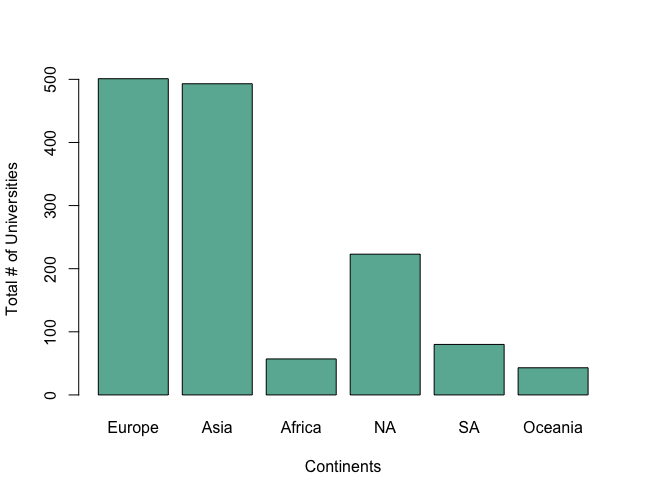
\includegraphics[width= 10cm]{bar chart continents.png}
  \captionof{figure}{Bar chart of Continents' Universities}
  \label{fig:test3}
\end{minipage}%
\begin{minipage}{.5\textwidth}
  \centering
  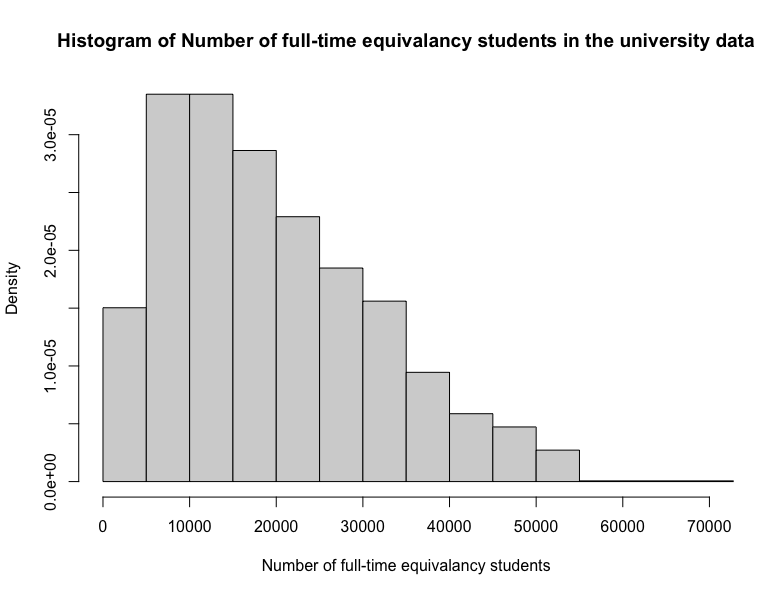
\includegraphics[width=10cm]{Rplot01.png}
  \captionof{figure}{Histogram of the density of the number of fulltime-efficiency students in a university}
  \label{fig:test4}
\end{minipage}
\end{figure}
\end{document}
